\chapter{Introdu\c{c}\~ao e teoria}

%\section{Motiva\c{c}\~ao}

% DIZER ALGO SOBRE COMO SERA O SISTEMA, COM BARRAS E CONEXOES E QUE FICA COMPLEXO SEM ANALISE DE FLUXO DE CARGA Mas como \'e possivel garantir o planejamento e opera\c{c}\~ao sistema de grandes propor\c{c}\~oes como esse? Para isso, \'e preciso saber o estado atual do sistema. Por\'em, n\~ao \'e vi\'avel medir todos os pontos de interesse. Isso seria custoso e tomaria muito tempo. 


%Para  como um todo \'e necessario que tenhamos ferramentas que nos ajudem a estimar o estado da rede 

%\section{Introdução à Teoria}
A ferramenta de an\'alise de sistemas de energia el\'etrica aqui discutida ser\'a a An\'alise de Fluxo de Pot\^encia. Essa an\'alise nos fornecer\'a um metodo de cálculo de importantes grandezas de todo o sistema, a partir de algumas grandezas conhecidas, ou seja, que podem ser medidas. Esta \'e uma ferramenta aplicada \`a um sistema est\'atico.  \cite{monticelli}
\section{Modelagem}
\label{SectionIntro}
Toda a rede ser\'a composta por ramos e barras, onde ramos s\~ao a representa\c{c}\~oes das linhas de transmiss\~ao e transformadores. As barras s\~ao n\'os do sistema e nesses pontos de interesse, pode-se medir fisicamente algumas grandezas, a depender do tipo de barra. S\~ao definidas quatro vari\'aveis \`a para cada k-ésima barra, correspondentes \`a tens\~ao e \`a inje\c{c}\~ao de
pot\^encia nesta barra, $V_k$, magnitude da tens\~ao nodal, $\theta_k$ angulo da tens\~ao nodal, $P_k$ inje\c{c}\~ao l\'iquida de pot\^encia ativa e $Q_k$ inje\c{c}\~ao l\'iquida de pot\^encia reativa. As barras s\~ao divididas em categorias como na tabela \ref{t_PQPVSlack} de acordo com as grandezas conhecidas e suas incognitas.
\begin{table}[]
\caption{Categoria das barras de acordo com variáveis conhecidas}
\begin{tabular}{@{}llll@{}}
\toprule
Tipo & Dados & Incógnitas & Caracteristicas \\ 
\midrule
$PQ$ & $P_k$,$Q_k$ & $V_k$,$\theta_k$  & Barra de carga \\
$PV$ & $P_k$,$V_k$ & $Q_k$,$\theta_k$  & Barra de geração\\
Referência (Slack) & $V_k$,$\theta_k$ & $P_k$,$Q_k$& Barra de geração em grandes fornecedoras \\ \bottomrule
\end{tabular}
\label{t_PQPVSlack}
\end{table}



\section{Formula\c{c}\~ao do problema b\'asico}
\label{SectionFormula}
\subsection{Injeção de potências}

Seja uma rede de energia gen\'erica que cont\'em um n\'umero de barras \textit{(NB)} arbitr\'ario. Para cada barra, \'e poss\'ivel escrever duas equa\c{c}\~oes de inje\c{c}\~oes de pot\^encia, como em \ref{Pk} e \ref{Qk}. Elas são obtidas ao aplicar Lei de Kirchhoff das correntes em todas as $NB$ barras do sistema.\\
\begin{equation}
    P_k = V_k \sum_{m\in \kappa} V_m (G_{km} cos\theta_{km} + B_{km}sen\theta_{km})
    \label{Pk}
\end{equation}
\begin{equation}
    Q_k = V_k \sum_{m\in \kappa} V_m (G_{km} sen\theta_{km} - B_{km}cos\theta_{km})
    \label{Qk}
\end{equation}
Portanto, em um sistema com \textit{NB} barras, \'e possivel obter $2.NB$ equa\c{c}\~oes.\\
Neste problema, utilizaremos como variáveis de estado, ou seja, nosso conjunto de incognitas que descreverão o sistema, as variáveis $V$ e $\theta$, representados em \ref{Vs} e \ref{TetaS}. Com esses valores resolvidos, \'e possível calcular todas as injeções de potência em todas as barras.\\
\begin{equation}
    V^S  = \left[ \begin{matrix} V_1^S & V_2^S & V_3^S & ... & V_{NB}^S  \end{matrix} \right]^T 
    \label{Vs}
\end{equation}

\begin{equation}
    \theta^S  = \left[ \begin{matrix} \theta_1^S & \theta_2^S & \theta_3^S &... & \theta_1^S  \end{matrix} \right]^T 
    \label{TetaS}
\end{equation}
Quando \ref{Vs} e \ref{TetaS} forem resolvidas, será possivel aplicar em \ref{Pk} e \ref{Qk} para se obter \ref{Pk_s} e \ref{Qk_s}, que será as injeções de potência para o estado atual da rede.
\begin{equation}
    P_k = V_k^S \sum_{m\in \kappa} V_m^S (G_{km} cos\theta_{km}^S + B_{km}sen\theta_{km}^S)
    \label{Pk_s}
\end{equation}
\begin{equation}
    Q_k = V_k^S \sum_{m\in \kappa} V_m^S (G_{km} sen\theta_{km}^S - B_{km}cos\theta_{km}^S)
    \label{Qk_s}
\end{equation}
Problema consiste em obter o estado $(V^S,\theta^S)$.\\
Com um simples algebrismo matemático, as equações \ref{Pk} e \ref{Qk} serão representas aqui como em \ref{Pk_balanceado} e \ref{Qk_balanceado}.
\begin{equation}
    P_k - V_k \sum_{m\in \kappa} V_m (G_{km} cos\theta_{km} + B_{km}sen\theta_{km}) = 0
    \label{Pk_balanceado}
\end{equation}
\begin{equation}
    Q_k - V_k \sum_{m\in \kappa} V_m (G_{km} sen\theta_{km} - B_{km}cos\theta_{km}) = 0
    \label{Qk_balanceado}
\end{equation}

%essas equaoces tem que dar 0 pois são dua coisas iguais

%dada uma rede qualquer, o nume de equacoes sera XXXX colocar 

%inserir tahbelas tipos de barras

%numero de equacoes = numero de incognitas e o sistema é LI. POrtante há solução

%do ponto de vista didático

\subsection{Matriz de Admitância}
Seja a matriz de admitância nodal $Y$ e ela se relacione com o vetor de tensões nodais $V$ e vetor de injeções de corrente nodais $I$ da forma como em \ref{Admitancia}.
\begin{equation}
    I = Y.V
    \label{Admitancia}
\end{equation}
A regra de formação dessa matriz $Y$ será dada por \ref{AdmitanciaElementosForaDiagonal} e \ref{AdmitanciaElementosDiagonal} (A dedução desse conjunto de formulas não será abordado neste trabalho).\\
A dimensão da matriz $Y$ será de $NB$x$NB$.\\
Para os elementos fora da diagonal principal, será o valor negativo da admitância série entre as duas barras, como em \ref{AdmitanciaElementosForaDiagonal}.
\begin{equation}
    Y_{km} = -y_{km}
    \label{AdmitanciaElementosForaDiagonal}
\end{equation}
Para os elementos na diagonal principal, será a soma das admitâncias conectadas à barra, como em \ref{AdmitanciaElementosDiagonal}, onde $\Omega_k$ é o conjunto de barras vizinhas da barra $k$.
\begin{equation}
    Y_{kk} = \sum_{m\in \Omega_k} \left(y_{km} + j\frac{b^{sh}_{km}}{2}\right)
    \label{AdmitanciaElementosDiagonal}
\end{equation}
Ainda, a matriz $Y$ será dividida em parte real(\ref{G}) e parte imaginária (\ref{B}). Dando origem às matrizes de condutância $G$ e susceptância $B$, usadas nas equações de injeção de potência \ref{Pk} e \ref{Qk}.
\begin{equation}
    G = \mathbb{R} (Y)
    \label{G}
\end{equation}
\begin{equation}
    B = \mathbb{I} (Y)
    \label{B}
\end{equation}



%\subsection{Subsistema 1}
%calcular v e teta faltando

%na barra de ref não falta nenhum
%na barra PQ falta 2 variaveis V e teta
%na barrade geraç~]a., PV, já conheco V, só falta teta


%grandezas conhecidas 
%2NPQ + NPV grandezas

%problemas tem solução

%como serao as equacçoes. Serão eq de injeções de pot ativa e reativa

%P espeficada 
%valor especificado na barra k - valor calculado = 0 

%\subsection{Subsistema 2}
%calcula P e Q faltando

%conhecendo os V e Tetas, calcula-se P e Q
%na barra PV vc calcula só Q
%na barra slack vc calcula P e Q

\section{Formula\c{c}\~ao do m\'etodo de Newton}
\label{SectionNewton}
O algoritmo de Newton é um método para calcular os zeros de funções reais de uma variável reais. Baseando em uma aproximação inicial arbitraria, $x^{(1)}$, tem-se \ref{Newton} para $n>1$. \cite{newton}
\begin{equation}
    x^{x+1} = x^{n} - \frac{f(x^{(n)}}{f'(x^{(N)}} = x^{n} - \Delta x
    \label{Newton}
\end{equation}
Fazendo $\Delta x = \frac{f(x^{(n)}}{f'(x^{(N)}}$ 
\begin{equation}
    x^{x+1} = x^{n} - \Delta x
    \label{Newton_Delta}
\end{equation}
\subsection{Aplicação do método de Newton em problemas de Fluxo de Potência}
Para solucionar o problema do Fluxo de Potência utilizando o método de Newton, é necessário estabelecer equações que relacionem o problema na forma de $f(x)=0$. A forma mais adequada, é utilizando as equações que modelam o balanceamento das injeções de potência \ref{Pk_balanceado} e \ref{Qk_balanceado}, mas desta vez elas não vão a $0$, pois ainda não estão resolvidas. Neste momento, igualaremos elas um $\Delta$, que é tão próximo de $0$ quanto se queira, como descrito nas equações \ref{Pk_balanceado_delta} e \ref{Qk_balanceado_delta}.\\
\begin{equation}
    \Delta P_k = P^{esp}_k - P^{calc}_k(V,\theta)= P^{esp}_k - V_k \sum_{m\in \kappa} V_m (G_{km} cos\theta_{km} + B_{km}sen\theta_{km})
    \label{Pk_balanceado_delta}
\end{equation}
\begin{equation}
    \Delta Q_k = Q^{esp}_k - Q^{calc}_k(V,\theta) = Q^{esp}_k - V_k \sum_{m\in \kappa} V_m (G_{km} sen\theta_{km} - B_{km}cos\theta_{km})
    \label{Qk_balanceado_delta}
\end{equation}
Onde:
\begin{itemize}
    
    \item $P^{esp}_k = P^G_k -P^C_k$ e $Q^{esp}_k = Q^G_k -Q^C_k$ que são os valores das injeções de potência ativa e reativa especificados para as barras.
    \item $P^{calc}_k(V,\theta)$ e $Q^{calc}_k(V,\theta)$ são calculados através das equações das potências nodais.
    \item $\Delta P_k$ e $\Delta Q_k$ são chamados de mismatches ou resíduos de potência ativa e reativa. 

\end{itemize}
Em termos práticos, para a resolução do sistema de equações $g(x) = 0$ pelo método de Newton, é necessário a determinação do vetor de correção do estado $\Delta x$ a cada iteração. Para cada iteração  $\nu$, $\Delta x$ é obtido através de \ref{Newton_aplicado} e verificado se a convergência ocorreu, isto é, se $|\Delta_x| < Tol$.\\
\begin{equation}
    g(x^\nu) = -J(x^\nu) . \Delta (x^\nu)
    \label{Newton_aplicado}
\end{equation}
Onde:\\
\begin{equation}
   g(x^\nu) = \left[ \begin{matrix} \Delta P^\nu \\ \Delta Q^\nu  \end{matrix} \right] 
    \label{g_x_nu}
\end{equation}
\begin{equation}
   \Delta (x^\nu) = \left[ \begin{matrix} \Delta \theta^\nu \\ \Delta V^\nu  \end{matrix} \right] 
    \label{delta_x_nu}
\end{equation}
\begin{equation}
   J (x^\nu) = - \left[ \begin{matrix} \frac{\partial (P)}{\partial \theta} & \frac{\partial (P)}{\partial V}  \\ \frac{\partial (Q)}{\partial \theta} & \frac{\partial (Q)}{\partial V}  \end{matrix} \right] 
    \label{Jacobiana}
\end{equation}
As submatrizes que compõem a matriz Jacobiana \ref{Jacobiana} são geralmente representadas por \ref{H}, \ref{N}, \ref{M} e \ref{L} e são obtidas equações das potências nodais \ref{Pk} e \ref{Qk}
\begin{equation}
   H = \frac{\partial (P)}{\partial \theta}
    \label{H}
\end{equation}
\begin{equation}
   N = \frac{\partial (P)}{\partial V}
    \label{N}
\end{equation}
\begin{equation}
   M = \frac{\partial (Q)}{\partial \theta}
    \label{M}
\end{equation}
\begin{equation}
   L = \frac{\partial (Q)}{\partial V}
    \label{L}
\end{equation}
Resultando em \ref{HNML_eq}.
\begin{equation}
    \left[ \begin{matrix} \Delta P^\nu \\ \Delta Q^\nu  \end{matrix} \right]  = \left[ \begin{matrix} H & N \\ M & L  \end{matrix} \right]^\nu . \left[ \begin{matrix} \Delta \theta^\nu \\ \Delta V^\nu  \end{matrix} \right] 
    \label{HNML_eq}
\end{equation}
As mastrizes H, N, M e L podem ter seus valores calculados utilizando as equações \ref{H_resolvido}, \ref{N_resolvido}, \ref{M_resolvido} e \ref{L_resolvido}.(As deduções das matrizes H, N, M e L podem ser encontradas em livros didáticos e, portanto, serão omitidas neste trabalho).\\

\begin{equation}
  \left\{    \begin{array}{lll}
                H_{kk} = \frac{\partial (P_k)}{\partial \theta_k} = -B_{kk}V_k^2 - V_k\sum_{m\in \kappa} V_m(G_{km} sen\theta_{km} - B_{km}cos\theta_{km})\\
                H_{km} = \frac{\partial (P_k)}{\partial \theta_m} = V_k V_m (G_{km} sen\theta_{km} - B_{km}cos\theta_{km})\\
                H_{mk} = \frac{\partial (P_k)}{\partial \theta_k} =-V_k V_m (G_{km} sen\theta_{km} + B_{km}cos\theta_{km})
            \end{array}\right.
    \label{H_resolvido}
\end{equation}

\begin{equation}
  \left\{    \begin{array}{lll}
                N_{kk} = \frac{\partial (P_k)}{\partial V_k} = G_{kk}V_k \sum_{m\in \kappa} V_m(G_{km} cos\theta_{km} + B_{km}sen\theta_{km})\\
                N_{km} = \frac{\partial (P_k)}{\partial V_m} = V_k(G_{km} cos\theta_{km} + B_{km}sen\theta_{km})\\
                N_{mk} = \frac{\partial (P_m)}{\partial V_k} =V_m(G_{km} cos\theta_{km} + B_{km}sen\theta_{km})
            \end{array}\right.
    \label{N_resolvido}
\end{equation}

\begin{equation}
  \left\{    \begin{array}{lll}
                M_{kk} = \frac{\partial (Q_k)}{\partial \theta_k} = -G_{kk}V_k^2 + V_k\sum_{m\in \kappa} V_m(G_{km} cos\theta_{km} + B_{km}sen\theta_{km})\\
                M_{km} = \frac{\partial (Q_k)}{\partial \theta_m} = -V_k V_m (G_{km} cos\theta_{km} + B_{km}sen\theta_{km})\\
                M_{mk} = \frac{\partial (Q_m)}{\partial \theta_k} =-V_k V_m (G_{km} cos\theta_{km} - B_{km}sen\theta_{km})
            \end{array}\right.
    \label{M_resolvido}
\end{equation}

\begin{equation}
  \left\{    \begin{array}{lll}
                L_{kk} = \frac{\partial (Q_k)}{\partial V_k} = -B_{kk}V_k +\sum_{m\in \kappa} V_m(G_{km} sen\theta_{km} - B_{km}cos\theta_{km})\\
                L_{km} = \frac{\partial (Q_k)}{\partial V_m} = V_k(G_{km} sen\theta_{km} - B_{km}cos\theta_{km})\\
                L_{mk} = \frac{\partial (Q_m)}{\partial V_k} =-V_m (G_{km} sen\theta_{km} + B_{km}cos\theta_{km})
            \end{array}\right.
    \label{L_resolvido}
\end{equation}
\subsection{Método de Newton desacoplado}
\label{SubsectionMetodoDeNewtonDesacoplado}
Como dito no tópico anterior, para cada iteração do método de Newton, deve-se resolver o sistema apresentado em \ref{HNML_eq}. Para isso, a matriz \ref{Jacobiana} deve ser fatorada, e dado que as submatrizes H, N, M e L, compostas pelos temos em \ref{H_resolvido}, \ref{N_resolvido}, \ref{M_resolvido} e \ref{L_resolvido}, variam à cada interação, é de se esperar que o esforço computacional seja grande.\\
Uma boa otimização será de evitar esse esforço computacional, que aumenta proporcionalmente ao número de ramos e baras analisados. Então, lança-se um artificio computacional que se baseia no desacoplamento das variáveis das partes ativa e reativa.

\subsubsection{Desacoplamento das variáveis}
\label{SubsectionMetodoNewtonDesacopladoVariaveis}
Especialmente para sistemas de extra alta tensão (acima de $230kV$) e ultra alta tensão (acima de $750kV$), pode se afirmar que há forte dependência entre os fluxos de potência ativa e os ângulos das tensões nas barras, assim como os fluxos de potência reativa e a magnitude das tensões nas barras \cite{fpdr}.\\
De maneira geral, pode-se observar que:
\begin{itemize}
    \item Variação de $\Delta P$ em $P$, implica em variação em $\Delta \theta$ e pequeno efeito em sobre a magnitude de tensão $(\Delta V \approx 0)$.
    \item Variação de $\Delta Q$ em $Q$, implica em variação em $\Delta V$ e pequeno efeito em sobre a ângulo da tensão $(\Delta \theta \approx 0)$.
\end{itemize}
Logo, pode-se escrever algebricamente \ref{DeltaPNewtonRapido} e \ref{DeltaQNewtonRapido}.
\begin{equation}
    \Delta P = H.\Delta\theta + \cancelto{0}{N.\Delta V} 
    \label{DeltaPNewtonRapido}
\end{equation}
\begin{equation}
    \Delta Q = \cancelto{0}{M.\Delta \theta} + L.\Delta V
    \label{DeltaQNewtonRapido}
\end{equation}
Com as submatrizes $N$ e $M$ sendo aproximadas para 0, para cada iteração $\nu$, o novo sistema será dado por \ref{HNML_eq_rapido} ao invés de \ref{HNML_eq}. As matrizes $H$ e $L$ são formadas pelas equações \ref{H_resolvido} e \ref{L_resolvido} permanecem as mesmas.
\begin{equation}
    \left[ \begin{matrix} \Delta P^\nu \\ \Delta Q^\nu  \end{matrix} \right]  = \left[ \begin{matrix} H & 0 \\ 0 & L  \end{matrix} \right]^\nu . \left[ \begin{matrix} \Delta \theta^\nu \\ \Delta V^\nu  \end{matrix} \right] 
    \label{HNML_eq_rapido}
\end{equation}

\subsubsection{Versão modificada do método de Newton desacoplado}
\label{SubsectionNewtonModificado}
Afim de se diminuir as não linearidades das equações, as submatrizes $H$ e $L$ , que antes eram formadas pelas equações \ref{H_resolvido} e \ref{L_resolvido}, nessa versão modificada, serão dividas por $V_i$, resultando em \ref{H_resolvido_Nmodificado} e \ref{L_resolvidoNmodificado}.
\begin{equation}
  \left\{    \begin{array}{lll}
                H_{kk}^{modificado}=\frac{H_{kk}}{V_k} = -B_{kk}V_k - \sum_{m\in \kappa} V_m(G_{km} sen\theta_{km} - B_{km}cos\theta_{km})\\
                H_{km}^{modificado} = \frac{H_{km}}{V_k} = V_m (G_{km} sen\theta_{km} - B_{km}cos\theta_{km})\\
                H_{mk}^{modificado} = \frac{H_{mk}}{V_m} = -V_k (G_{km} sen\theta_{km} + B_{km}cos\theta_{km})
            \end{array}\right.
    \label{H_resolvido_Nmodificado}
\end{equation}
\begin{equation}
  \left\{    \begin{array}{lll}
                L_{kk}^{modificado} = \frac{L_{kk}}{V_k} = -B_{kk} +\frac{\sum_{m\in \kappa} V_m(G_{km} sen\theta_{km} - B_{km}cos\theta_{km})}{V_k} \\
                 L_{km}^{modificado} = \frac{L_{km}}{V_k} = (G_{km} sen\theta_{km} - B_{km}cos\theta_{km})\\
                L_{mk}^{modificado} = \frac{L_{mk}}{V_m} =-(G_{km} sen\theta_{km} +B_{km}cos\theta_{km})
            \end{array}\right.
    \label{L_resolvidoNmodificado}
\end{equation}
De forma matricial, pode-se reescrever as equações \ref{DeltaPNewtonRapido} e \ref{DeltaQNewtonRapido} com as equações modificadas \ref{H_resolvido_Nmodificado} e \ref{L_resolvidoNmodificado} resultando em \ref{DeltaPNewtonModificado} e \ref{DeltaQNewtonModificado}. 
\begin{equation}
    \frac{\Delta P}{V} = H^{modificado}.\Delta\theta
    \label{DeltaPNewtonModificado}
\end{equation}
\begin{equation}
    \frac{\Delta Q}{V} = L^{modificado}.\Delta V
    \label{DeltaQNewtonModificado}
\end{equation}

\subsubsection{Método de Newton desacoplado rápido}
\label{SubsubsectionDesacopladoRapido}
A otimização usada no Método de Newton desacoplado rápido será baseada em algumas aproximações.\\
São elas:
\begin{itemize}
    \item $\theta_{km}$ pequeno $(cos(\theta_{km})\approx 1$
    \item $B_{km}\gg G_{km}sen(\theta_{^km})$
    \item $B_{kk}V_K^2\gg Q_k$
    \item $V_k \approx 1pu$
\end{itemize}
As condições de contorno devem ser verdadeiras para que haja convergência. Se todas as condições são cumpridas, pode-se constituir duas novas matrizes, $B'$ e $B''$ que serão as novas aproximações de $H^{modificado}$ e $L^{modificado}$. São dadas por \ref{Blinha} e \ref{Bduaslinhas}.
\begin{equation}
  \left\{    \begin{array}{lll}
                B'_{kk}=-B_{kk}\\
                B'_{km}=-B_{km}\\
                B'_{mk}=-B_{km}
            \end{array}\right.
    \label{Blinha}
\end{equation}
\begin{equation}
  \left\{    \begin{array}{lll}
                B''_{kk}=-B_{kk}\\
                B''_{km}=-B_{km}\\
                B''_{mk}=-B_{km}
            \end{array}\right.
    \label{Bduaslinhas}
\end{equation}
Substituindo \ref{H_resolvido_Nmodificado} e \ref{L_resolvidoNmodificado} por \ref{Blinha} e \ref{Bduaslinhas}, respectivamente, as equações do método desacoplado rápido serão dadas por \ref{DeltaPNewtonModificadoRapido} e \ref{DeltaQNewtonModificadoRapido}.
\begin{equation}
    \frac{\Delta P}{V} = B'.\Delta\theta
    \label{DeltaPNewtonModificadoRapido}
\end{equation}
\begin{equation}
    \frac{\Delta Q}{V} = B''.\Delta V
    \label{DeltaQNewtonModificadoRapido}
\end{equation}

\section{Algoritmo implementado}

Aqui será utilizado um algoritmo discutido nos slides do Professor Castro. \cite{castro}.

\subsection{Método de Newton}
\label{SubsectionMetodoNewton}
\begin{enumerate}
    \item   O contador de iterações é inicializado $\nu = 0$.   Escolhe-se condições de contorno iniciais para as magnitudes das tensões nodais nas barras $PQ$ e ângulos de fase das tensões nodais nas barras $PQ$ e $PV$, onde não houver esse valor previamente estabelecido.
            O vetor $x$ pode ser montado como em \ref{X}.
            \begin{equation}
            x  = \left[ \begin{matrix} \theta^0 & V^0  \end{matrix} \right]^T 
            \label{X}
            \end{equation}
    \item   Calcula-se $P_k(V_\nu, \theta)$ para as barras $PQ$ e $PV$.\\
            Calcula-se $Q_k(V_\nu, \theta_\nu)$ para as barras $PQ$.
            Calcula-se os respectivos mismatches de potência \ref{delta_x_nu}.
    \item   Testa-se a convergência: Se $max \{|\Delta P_k^\nu|\}_k=PQ$ , $PV\leq \varepsilon P$ e $max \{|\Delta Q_k^\nu|\}_k=PQ \leq \varepsilon P$\\
            Então processo iterativo convergiu para a solução $[\theta ^\nu V^\nu]^T$. Pular para o passo $7$.\\
            Senão, prosseguir para passo $4$.
    \item   \label{ItemJacobiana} Calcula-se a matriz Jacobiana como em \ref{Jacobiana}
    \item   Calcula-se as correções resolvendo o sistema \ref{HNML_eq} e determina-se nova solução $(V^{\nu + 1},\theta^{\nu + 1})$
    \item   Incrementa-se contador de iterações $\nu = \nu + 1$ e volta-se ao passo 2.
    \item   Calcula-se $P_k$ para a barra de referência e $Q_k$ para as barras de referência e $PV$.
\end{enumerate}

\subsection{Método de Newton desacoplado}

Para o método de Newton desacoplado, segue-se os mesmos passos descritos na subseção \ref{SubsectionMetodoNewton}, com diferença apenas do ítem \ref{ItemJacobiana}. Nesse caso a matriz Jacobiana não seguirá a formação descrita em \ref{Jacobiana} e sim a forma descrita em \ref{HNML_eq_rapido}.\\
Note que, ao considerar o sistema desacoplado como em \ref{DeltaPNewtonModificado} e \ref{DeltaQNewtonModificado}, e zerar as submatrizes $M$ e $N$, obtem-se um ganho de performance em cada iteração, pois há menos calculos a se fazer.\\
Para a versão modificada do método desacoplado, descrito na seção \ref{SubsectionNewtonModificado}, tem-se todas as equações que compõe as submatrizes $H$(\ref{H_resolvido_Nmodificado}) e $L$(\ref{L_resolvidoNmodificado}) serão divididas por $V_i$, assim como os \textit{mismatches} de potência, como em \ref{DeltaPNewtonModificado} e \ref{DeltaQNewtonModificado}. Então, nesse método, ainda há melhor performance como no método desacoplado, onde as submatrizes $M$ e $N$ são zeradas, além de reduzir o grau de não linearidades, ao dividir todo o sistema por $V_i$.\\
Para a versão desacoplada rápida, a única diferença reside, também, na simplificação da formação da matriz Jacobiana. A formação desta matriz respeitará as equações descritas em \ref{Blinha} e \ref{Bduaslinhas}, desde que suas condições descritas na subseção \ref{SubsubsectionDesacopladoRapido} sejam válidas.\\
Os passos para o Método de Newton desacoplado rápido estão sumarizados na figura \ref{FigNewtonRapidoFluxograma}. \cite{fpdr}.
\begin{figure}[!htb]
\caption{Método de Newton desacoplado rápido - Fluxograma}
 \centering % para centralizarmos a figura
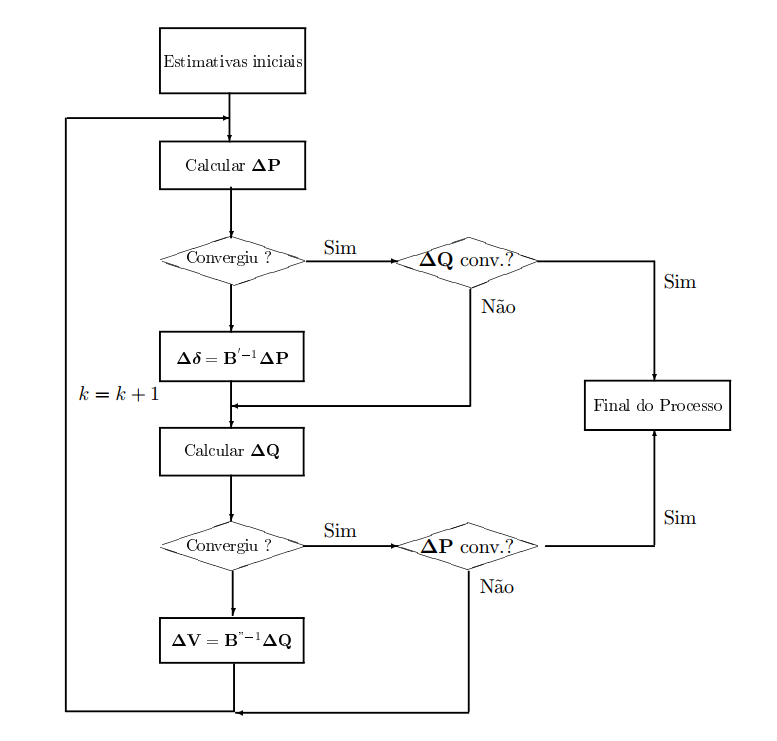
\includegraphics[width=12cm]{figuras/fluxograma.PNG} 
\label{FigNewtonRapidoFluxograma}
\end{figure}